% Created by Carlo Occhiena, 2023
% Engine: XELATEX
% Version: TeX 2019

\documentclass{article}

% PACKAGES
\usepackage[utf8]{inputenc}
\usepackage{amsmath} % provides many mathematical environments & tools
\usepackage{amssymb} % to display \varnothing symbol
\usepackage{array} % to manage table alignment
\usepackage{changepage} % dinamically change a page layout
\usepackage{geometry} % to manage dynamic page layout
\usepackage{graphicx} % to handle images
\usepackage{makecell} % to manage multiline cells
\usepackage[document]{ragged2e} %% to manage text alignment
\usepackage{parskip} % to manage paragraph spacing
% this has to be the last package ever  
\usepackage{hyperref} % clickable URLs

\graphicspath{ {./images/} } % tells the program what folder to find the images in

% USER CUSTOMIZATION
\renewcommand{\arraystretch}{1.5} % add height to tables

% FUNCTIONS 


\title{The Statistics Handbook \\ 
    \normalsize Version 0.1}
\author{ Carlo Occhiena }
\date{ Jan 2023 }


\begin{document}

\maketitle
% \centerline \LaTeX{}
\tableofcontents
\clearpage

\section{Scope of this handbook}
We are used to talking generally about mathematical skills, thinking perhaps of derivatives, integrals, theorems, and graphs of functions. 

Often we do that in an abstract way, as if they were certainly logical elements, but with just specific applications. Instead, we forget that not only are mathematical elements present in every single action, but that quantitative sciences are components of everyday life.

Specifically, I believe that statistics is among all the mathematical sciences the most fascinating because of the vastness and incredible opportunities for its application. 

Every decision we make can be traced back to statistical phenomena, either innate (such as fear of the dark, because in the dark increases the likelihood of dangerous animals) or conscious (today I think it's likely to rain, so I'll take my umbrella). 

On the other hand, approaching even basic statistical calculations (e.g., the infamous probability of winning the lottery) requires nontrivial skills in order to apply concepts and formulas that are not always complex but certainly have dissimilar results if used thoughtlessly. I claim for certain that worse than the lack of mathematical thinking is the misuse of mathematical thinking. This paper of mine is also in fact intended to combat my limitations through study and applications. 

In this handbook, I wanted to create a path from the basics, including terminology (often one of the main obstacles for the laymen approaching the subject), to formulations of hypotheses, validations, and verification of formulas.

The path was constructed by consulting a large number of sources, cited in the appendix, and during long months of study and in-depth proof of the results and evidence, precisely because first and foremost I wanted to verify my own expertise, even before, of course, I could write about it. 

Before releasing this publication, which is distributed under a Creative Common and Free Culture license, I asked for a check from eminent acquaintances with important academic and working backgrounds. I would like to endlessly thank all of them (their names can be found in the appropriate section). Nevertheless, I am staying receptive to additions, insights and corrections, taking full responsibility for any shortcomings and errors, certainly reported in good faith.

Happy reading! 

Carlo, 4th of January 2023.

\subsection{Versioning \& Contributions}
\begin{itemize}
    \item Version 0.1 is the first release ever published and distributed online. It's the version written and verified personally by me but does not include any third-party contributions or revisions. 
    \item I plan to submit the handbook to several SME (Subject Matter Experts). 
    \item Each contribution will be indicated in the Acknowledgments section. 
    \item The feedback from each SME will help raise the version by 1/10, so that with 9 revisions it will progress to version 1.0 of the document.
    \item Contributions are free and welcome, you can contact me via \href{https://www.linkedin.com/in/carloocchiena/}{Linkedin}. 
\end{itemize}


\subsection{\LaTeX{} \& Open Source Repository}
In addition to being distributed under a Free Culture CC BY 4.0 license, all materials related to this handbook are available in the GitHub repository at the link: \href{https://github.com/carloocchiena/the_statistics_handbook}.

This also includes the \LaTeX{} source of this handbook and an Excel with several exercises and applied formulas. This could therefore also be helpful to students and those who want to use this handbook for practical purposes. 

\clearpage

\section{Core Concepts}
\subsection{Let's start from a question}
“What is data?”

Data are collected observations and information about a given phenomenon.

“What is statistics?”

Statistics Is the discipline that concerns the collection, organization, analysis, interpretation, and presentation of data.

“What is a statistical variable?”

It’s the specific characteristic being analyzed among the statistical units on which the statistical analysis is focused on, such as “age” from all the data that may be related to the object “person”. Classification of variables and their measure of scale is paramount to set up the analytical process of statistical analysis. 

\subsection{Property and type of data}

We should not think that the data is solely a numerical value. There is a multitude of data types, each with specific characteristics. 

\subsubsection{Continuous vs Discrete}
Discrete means it can only take certain values. There are no “in-between” values. 

Discrete data is the number of people: there could be 1 person or 2 people, but not 1,5 people or 0,99 people. 
Discrete data are the possible value of rolling a die: 1,2,3,4,5,6 and not 6.5 or 1.5

Continuous means there is an infinite amount of value in between each data point.

Continuous data is the height or weight of a person.
Continuous data are temperature records. 
 
\subsubsection{Nominal vs Ordinal}
Nominal data is classified without a natural order or rank. Nominal data can’t be clearly sorted. 
Nominal data can’t be “ordered” (from which the term “ordinal”).

Nominal data are animal species: lizard, dog, cat, or the list of ingredients on a recipe.

Ordinal data is data that has a natural order or rank. 
Ordinal data can be sorted and ordered. 
Ordinal data doesn’t have to be numeric. For example, hot, mild, cold - or even top, low, bottom, can be data attributes that can be ordered and then being considered ordinal. 
Ordinal data are the seat numbers on a train. 

\subsubsection{Structured vs Unstructured}
Structured data is highly specific and stored in a predefined format. It has its own structure.
Examples are JSON or Excel files, SQL databases. 

Unstructured data is data that does not have a specific or well defined format. 
Unstructured data are audio data, text data, video data. 

Do not confuse “file format” with “formatted data”. 
Just because text is in a PDF format doesn't make it structured data. 

\subsubsection{Statistical Variables and their properties}
\paragraph{Qualitative Statistical Variables}\mbox{} \\
\mbox{} \\

Qualitative statistical variables are variables whose values are not numbers but modes, or categories. 

Examples are: “male” or “female”, “education”, “marital status”, “ethnicity” and such.

Those categories have to be exhaustive and mutually exclusive - a datapoint can’t be both “male” and “female” or both “asian” and “european”. This is a specific problem that may occur in the data preparation and data gathering phase. 

Qualitative statistical variables can be classified further in:

\textbf{Dichotomic:} variables that have only two kinds of mutually exclusive categories,  such as “male” or “female” or “alive” or “dead”.

\textbf{Nominal:} variables that have no logical order, are not comparable and not exclusive to each other. Examples of nominal variables are “transportation used for work” or “sport played”.

\textbf{Ordinal:} variables that have a logical predefined order, but yet can’t be classified as quantitative. 
Example is “education”; High School is surely lower than University, but of how much? 
And how far is a MsC from a PhD? They are clearly different, but this difference can’t be clearly measured. 

    \begin{itemize}
        \item \textbf{Linear ordinal:} they have a clear start and end, such as size “S M L XL”.
        \item \textbf{Cyclical ordinal:} they have no clear start and end and their order is based on convention (such as week days: weeks starts both on Monday, or on Sunday. Seasons).
    \end{itemize}

\paragraph{Quantitative statistical variables}\mbox{} \\
\mbox{} \\

Quantitative statistical variables are expressed by a numerical quantity.
Quantitative data is naturally ordinable and comparable. 

Quantitative data can be further classified in: 

    \begin{itemize}
        \item \textbf{Interval data:} datapoint are expression of a specific point of the dataset (such as result of a test, QI, temperature).
        \item \textbf{Ratio scale data:} data that is expressed by a rate, such as age and weight.
    \end{itemize}

\paragraph{Parametric vs Nonparametric}\mbox{} \\
\mbox{} \\

\textbf{Parametric tests}
\begin{itemize}
    \item Parametric tests assume the presence of distributions of approximately normal type.
    \item They involve continuous or interval-type variables and a fairly large sample size.
    \item They assume homogeneity of variances (homoscedasticity).
    \item They assume estimation of parametric data such as mean, variance and standard deviation.
\end{itemize}

These tests have higher statistical power because they provide a higher probability of correct rejection of an incorrect statistical hypothesis. 

\textbf{Nonparametric tests}\mbox{} \\
Nonparametric tests don’t imply any kind of distribution and don’t imply any kind of parametric estimation such as mean, variance and standard deviation (because, for example, such measures are not estimable).

Nonparametric tests should be preferred whenever the dataset is not distributed in a normal (gaussian distribution) way, or, in any case, this specificity is not being demonstrated. A typical example is whenever the dataset is too small to prove a parametric distribution.

\paragraph{Homoscedasticity vs Heteroscedasticity}\mbox{} \\ 
\mbox{} \\

\textbf{Homoscedasticity} means that all random variables in the dataset have the same finite variance.

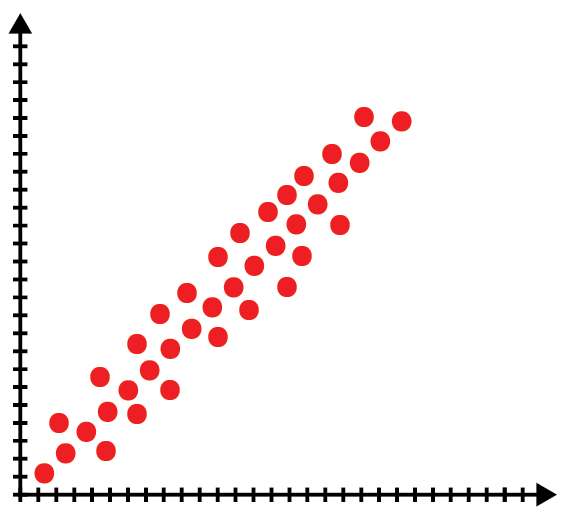
\includegraphics[width=3cm, height=3cm]{homoscedasticity}

\textbf{Heteroscedasticity}  means that not all random variables in the database have the same finite variance.

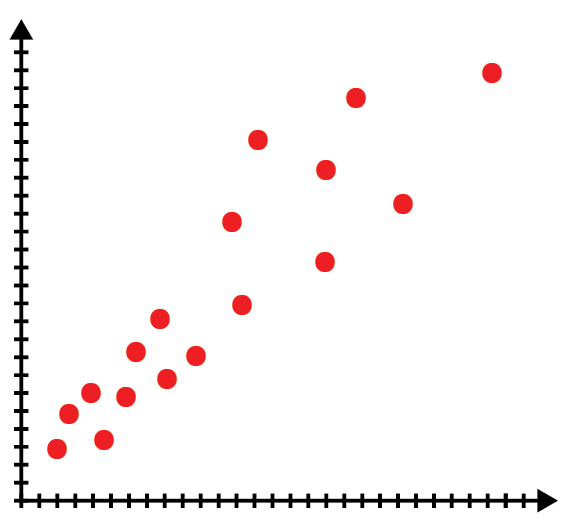
\includegraphics[width=3cm, height=3cm]{heteroscedasticity}

\subsection{Population vs Sample}

\textbf{Population} consists of the representation of every member of a given group or of the entire available data set.
Examples are all the students of a class or all the animals of a specific national park.

\textbf{Sample} refers to a subset of the entire data set. 
For example, the first 10 students of a class or the top 3 predators from a specific national park.

Population and Sample are data definitions that are heavily dependent from the context.

When analyzing data related to a population, it is necessary to include a statistically relevant sample. A representative sample. 
Sample sizes are a well studied science. 
For example 300 is a representative sample out of a population of 1000 students.

Use “population” when:
\begin{itemize}
    \item It’s known the dataset is related to the entire population.
    \item A generalization to a wider, larger population is not interesting.
\end{itemize}

Use “sample” when:
\begin{itemize}
    \item It’s known the dataset is related to a subset of the whole dataset.
    \item A generalization to a wider, larger sample or population is interesting
\end{itemize}

Rule of thumb: statisticians primarily work with samples. Real-world data can be overwhelmingly large.

\subsection{Parameters vs Statistics vs Hyperparameters}

\textbf{Parameters} describe the properties of the entire population.

\textbf{Statistics} describe the properties of a sample.

\textbf{Hyperparameters}\footnote{even if slightly out of context this is added for clarity and significance} (used in modeling and machine learning processes) are instead tuning values. Hyperparameters are set before the model is trained and are not coming from the dataset. 

\paragraph{Hat symbols over variables ($\hat{}$)}\mbox{} \\ 
\mbox{} \\
The estimated or predicted values in a regression or other predictive model in statistics are referred to as “hat values”. 

$\hat{y}$: $y$ is the outcome or dependent variable in the model equation, the "hat" symbol ($\hat{}$) placed over the variable name is the statistical designation of an estimated value.


\subsection{Descriptive and inferential statistics}

\textbf{Descriptive statistics} is a part of statistics that aim to describe data. It is used to summarize the attribute of a dataset, using measures such as Measures of Central Tendency or Measures of Dispersion.

\textbf{Inferential statistics} is a part of statistics that is used to test and validate assumptions over a dataset by analyzing a sample, using methods such as Hypothesis Testing or Regression Analysis.

\subsection{Binomial Distribution}
the binomial distribution with parameters n and p is the discrete probability distribution of the number of successes in a sequence of n independent experiments, each asking a yes–no question, and each with its own Boolean-valued outcome: success (with probability $p$) or failure (with probability $q=1-p$). 
A single success/failure experiment is also called a Bernoulli trial. 
A sequence of outcomes is called a Bernoulli process; for a single trial, i.e., $n = 1$, the binomial distribution is a Bernoulli distribution. 
The binomial distribution is the basis for the popular binomial test of statistical significance.

\subsubsection{Binomial Coefficient}
Binomial Coefficient is a natural number as defined starting from a pair of natural numbers, usually named $n$ and $k$. 
Binomial Coefficient represents the number of sub-groups of $k$ elements that could be made out of a dataset of $n$ objects.

\subsection{Measurement of Central Tendency}
\textbf{Central tendency} is defined as “the statistical measure that identifies a single value as representative of an entire distribution.” It aims to provide an accurate description of the entire data. It is the single value that is most typical/representative of the collected data.

\subsubsection{Mean}
Mean is generically expressed as:

$\frac{\text{sum of all data points}}{\text{number of data points}}$

And, more specifically, with the formula:\\
\mbox{} \\

${\displaystyle {\bar{x}}={\frac{1}{n}}\left(\sum _{i=1}^{n}{x_{i}}\right)={\frac{x_{1}+x_{2}+\cdots +x_{n}}{n}}}$

\mbox{} \\

Mean is the same concept of “average”, but average is generally used in arithmetic, while “mean” is expressingly considering the central point among a dataset in statistics. Arithmetic Mean is equal to average, while Harmonic or Geometric Mean have different meanings. 

Mean can be expressed also with symbols:\\
$\mu$ called MU or even with $\bar{x}$ ("ex bar").

In the specific context of statistical studies, 
$\bar{x}$ is used for mean over sample.\\
$\mu$ is used for mean over the entire population.\\

\textbf{Arithmetic Mean}
It's the simplest and most common type of  average, expressed as the sum of all data points over the count of data points.

\textbf{Weighted Mean}
It's similar to the arithmetic mean, except the fact that each of the data point contributes to the computation with its own weight factor.

$ \displaystyle \mu(x) = \frac{\sum \limits ^{k} _{i=1} x_i * n_i}{N}$

For example, let's calculate the average weight of an apple, given that you have many apples with different weight clusters.

\begin{center}
\begin{tabular}{|c|c|}
\hline
Apple (n) & Weight (g) \\ \hline
8 & 200 \\ 
3 & 250 \\ 
8 & 100 \\
\hline
\end{tabular}
\end{center}

The weighted mean would be then: $\frac{((8*200)+(3*250)+(8*100))}{(8+3+8)} = 165.75$ grams.  

\textbf{Truncated Mean}
A truncated mean or trimmed mean is a statistical measure of central tendency, much like the mean and median. It involves the calculation of the mean after discarding given parts of a probability distribution or sample at the high and low end, and typically discarding an equal amount of both. 
This number of points to be discarded is usually given as a percentage of the total number of points, but may also be given as a fixed number of points.

High and low end data points are called "outliers" (a data point that differs significantly from other observations).

\subsubsection{Mode}
The mode is the value occurring most often in a dataset.

$dataset = 8, 5, 4, 27, 35, 8, 29$
$mode = 8$

$dataset = 8, 5, 4, 27, 35, 8, 29, 35$
It’s a bi-modal dataset, mode being 35 and 8

$dataset =  5, 4, 27, 35, 8, 29$
$mode = \varnothing $

\subsubsection{Median}
The median is the central value of an ordered dataset.

Odd number of items dataset:\\
16, 18, 21, 27, 32, 33, 91\\
median = 27

Even number of items dataset:\\
16, 18, 21, 27, 32, 32, 33, 91\\
median = $\frac{(27 + 32)}{2} = 29.5$ 

\textbf{When to use mean, median and mode}

\begin{center}
\begin{tabular}{|l|c|c|c|}
\hline
DATASET & MEAN & MEDIAN & MODE \\ \hline
\textbf{Continuous} & YES & YES & YES \\ 
\textbf{Discrete} & YES & YES & YES \\ 
\textbf{Nominal} & MAYBE & NO & YES \\
\textbf{Ordinal} & MAYBE & YES & YES \\
\textbf{Numeric} & YES & YES & YES \\
\textbf{Non-numeric} & NO & YES & YES \\ 
\hline
\end{tabular}
\end{center}

\subsection{Measurement of Dispersion}
Measures of dispersion can be defined as positive real numbers that measure how homogeneous or heterogeneous the given data is. 

The most common measurements of dispersion are Variance and Standard Deviation. 

\subsubsection{Variance}
Variance represents the positive distance from a single datapoint for the mean of the dataset. The positive distance is made thanks to the exponential factor applied to the distance of each datapoint. 
The exponential factor also magnifies values that are more far from the mean in respect to smaller values, allowing to better understand their impact on the dataset. 

Variance is represented by: $\sigma ^{2}$ (when referred to population), ${\displaystyle s^{2}}$ (when referred to sample), ${\displaystyle \operatorname {Var} (X)}, {\displaystyle V(X)}, or {\displaystyle \mathbb {V} (X)}$

\subsubsection{Standard Deviation}
Standard Deviation is the square root of Variance and it’s represented with the Greek $\sigma$ or the letter $s$.

Being square rooted, the SD returns a value that has again the same scale of our dataset, hence allowing for better comparisons and understanding. 

Mean, Variance, and Standard Deviation, are closely linked together. 

\begin{center}
\begin{tabular}{|m{2cm}|c|c|}
\hline
& POPULATION (N) & SAMPLE (n) \\ \hline
&&\\[-1em]
Mean & $\displaystyle \mu = \frac{\sum\limits _{i=1}^{N} x_{i}}{N}$ & $\displaystyle \bar{x} = \frac{\sum\limits _{i=1}^{n} x_{i}}{n}$ \\[25pt]
Variance & $\displaystyle \sigma^2 = \frac{\sum\limits _{i=1}^{N} (x_{i} - \mu)^2}{N}$ & $\displaystyle s^2 = \frac{\sum\limits _{i=1}^{n} (x_{i} - \bar{x})^2}{n-1}$ \\[25pt]
Standard Deviation & $\displaystyle \sigma = \sqrt{\sigma^2}$ & $\displaystyle s = \sqrt{s^2}$ \\[25pt] 
\hline
\end{tabular}
\end{center}

\paragraph{Bessel's Correction}\mbox{} \\ 
\mbox{} \\

Why does sample variance have n-1 as denominator?

That’s a good question, that leads to a non-trivial answer. 

From a mathematical point of view, the -1 correction factor is called Bessel’s correction and it’s used to correct the tendency (that can be demonstrate mathematically or even empirically with a relatively small number of experiment over a dataset) that the biased estimator has a tendency to undershoot (and never to overshoot) the parameter being estimated.  

It is possible to think of the Bessel correction as the degrees of freedom of the vector of residuals. When the sample standard deviation is calculated from a sample of n values, sample mean is used which has already been calculated from that same sample of n values. The calculated sample mean has already taken into account one of the degrees of freedom of variability (which is the mean itself) that is available in the sample.

Let's approach the topic with an example: we have a table with 10 dice rolls; we know the result of each die, the overall average of the dataset.
How many elements can we make unknown in our dataset, without altering the goodness of the information we have?
Only one. By eliminating the result of one die roll, we are still able to reconstruct it through the mean of the experiment and the remaining values.
But by eliminating more than one value, we are forced to add approximation, thus invalidating the info we possess.
This is why we can link Bessel correction to degrees of freedom. 

\subsection{Quartiles and IQR}
In statistics, a quartile is a type of quantile which divides the number of data points into four parts, or quarters, of more-or-less equal size. The data must be ordered from smallest to largest to compute quartiles; as such, quartiles are a form of order statistic. 

\textbf{Quartiles:}
\begin{itemize}
    \item Quartile zero (Q0) corresponds to the first value of the ordered dataset.
    \item The first quartile (Q1) is defined as the middle number between the smallest number (minimum) and the median of the data set. It is also known as the lower or 25th empirical quartile, as 25\% of the data is below this point.
    \item The second quartile (Q2) is the median of a data set; thus 50\% of the data lies below this point.
    \item The third quartile (Q3) is the middle value between the median and the highest value (maximum) of the data set. It is known as the upper or 75th empirical quartile, as 75\% of the data lies below this point.
    \item Quartile four (Q4) corresponds to the last value of the ordered dataset.
\end{itemize}

\paragraph{IQR - Interquartile Range}\mbox{} \\
\mbox{} \\
IQR is a measure of statistical dispersion and it is defined as the difference between Q3 and Q1.

As an example, having an ordered dataset as following:\\
Dataset = 1, 2, 3, 5, 8, 8, 9, 10, 15\\
Q0: 1\\
Q1: (2 + 3) / 2 = 2.5 (median of first half; 25th percentile).\\
Q2: 8 (median; 50th percentile).\\
Q3: (9+10)  /2 = 9.5 (median of second half;75th percentile).\\
Q4: 15\\

Range = Q4 - Q0 = 15 - 1 = 14

IQR = Q3 - Q1 = 9.5 - 2.5 = 7

\subsection{Linear Regression}
Linear regression attempts to model the relationship between two variables by fitting a linear equation to observed data. The dependent variable $y$ is also called response variable. The independent variable $X$ is also called explanatory or predictor variables. \\
The resultant is a straight line intersecting the cartesian plane, attempting to minimize the distance (least-squares optimization) between actual output values so that hypothetical predicted values can be estimated.

Linear regression is a mathematical function based on the equation of the line:

$\displaystyle {Y_{i}=\beta _{0}+\beta _{1}X_{i}+u_{i}}$

Where:\\
\begin{itemize}
    \item $\displaystyle i$ ranges between observations, $\displaystyle i=1,\ldots,n.$
    \item $\displaystyle Y_{i}$ is the dependent (response) variable.
    \item $\displaystyle X_i$ is the independent (explanatory) variable.
    \item $\displaystyle \beta _{0}+\beta _{1}X$ is the regression function.
    \item $\displaystyle \beta _{0}$ is the line intercept (the value of $y$ when $x = 0$).
    \item $\displaystyle \beta _{1}$ is the line angular coefficient.
    \item $\displaystyle u_{i}$ is the statistical error.
\end{itemize}

Linear regression is a fundamental analysis of statistics, both because of its simplicity, interpretive immediacy and breadth of application cases.

Before attempting to fit a linear model to observed data, a modeler should first determine whether or not there is a relationship between the variables of interest. This does not necessarily imply that one variable causes the other, but that there is some significant association between the two variables. \\
A scatterplot can be a helpful tool in determining the strength of the relationship between two variables. \\
If there appears to be no association between the proposed explanatory and dependent variables (i.e., the scatterplot does not indicate any increasing or decreasing trends), then fitting a linear regression model to the data probably will not provide a useful model. \\ 
A valuable numerical measure of association between two variables is the correlation coefficient, which is a value between -1 and 1 indicating the strength of the association of the observed data for the two variables.

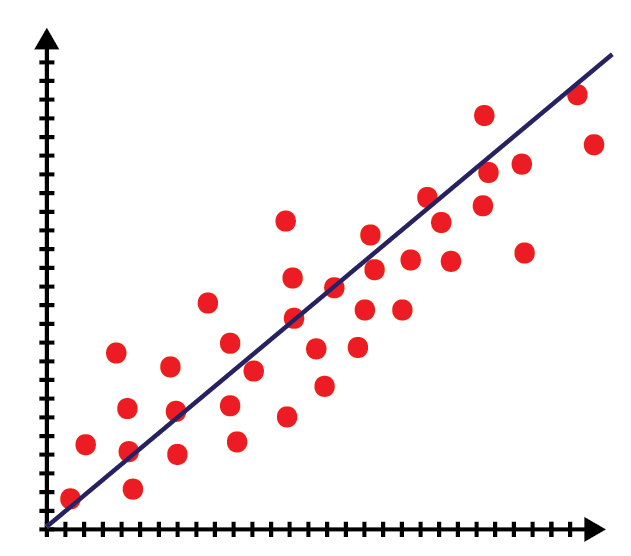
\includegraphics[width=3cm, height=3cm]{regression_chart}

\paragraph{Parameter estimations in the bivariate case}\mbox{} \\
\mbox{} \\
Generalizing the regression line equation, one can, in the case of the two-variable problem, start from:

$\hat{y} = mx + b +\varepsilon_{i}$,

Where:
\begin{itemize}
    \item $\hat{y}$ is the dependent (response) variable.
    \item $m$ is the line angular coefficient.
    \item $b$ is the line intercept.
    \item $\varepsilon_{i}$ is the statistical error.
\end{itemize}

At this point, the regression problem results in the determination of $m$ and $b$ so as to express the functional relationship between $y$ and $x$ as best as possible.

$\displaystyle m = \frac{n \sum{xy} - \sum{x}\sum{y}}{n\sum{x^2} - (\sum{x})^2}$ \\ \mbox{} \\
\mbox{} \\
$\displaystyle b = \frac{\sum{y} - m\sum{x}}{n}$

\clearpage
\section{Data Visualization}
Data visualization (data viz) is the graphical representation of data. 
The main goals of data visualization are to make the phenomena within the dataset more evident, convey the embedded information in the analysis more efficiently, and reinforce cognitive aspects of the provided study (e.g., ease of reporting, memorability).

While data visualization pertains to the field of science and statistics, it has also taken on cross-cutting significance in purely artistic or design-related contexts.

Data visualization  is so relevant that it could be considered a discipline within a discipline, with a deep vertical of study and insight that spans mathematical, scientific, statistical, cognitive, and humanistic domains. 

The recent spread of data science has made data viz even more important.

However, this paper will be limited to exploring some of the best-known forms of graphical representation in the field of statistics, and some of their properties.

\subsection{Scatter Plot}
A scatter plot is a type of plot or mathematical diagram using Cartesian coordinates to display values for typically two variables for a set of data. Every data point is displayed as a dot.

Scatter plot has its most significance with continuous distributions. 

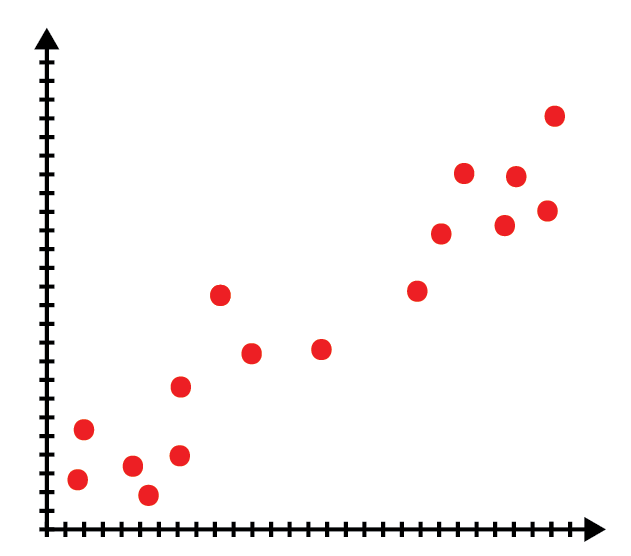
\includegraphics[width=3cm, height=3cm]{plot_chart}

\subsection{Line Chart}
Line charts show the evolution of a continuous variable (often over a time horizon).
A line chart is a way of plotting data points on a line. 
It is used to show trend data, or the comparison of two data sets.

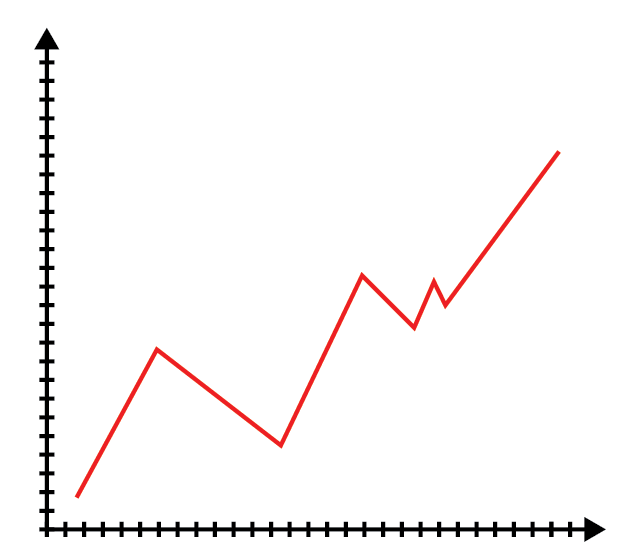
\includegraphics[width=3cm, height=3cm]{line_chart}

\subsection{Dot Plot}\footnote{In some texts, also called Line Plot.}
Dot plot is a way to display data frequency piled over data points and along a number line. 

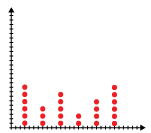
\includegraphics[width=3cm, height=3cm]{dot_plot}

\subsection{Histograms}
A histogram is a bar chart that groups continuous data into ranges. Ranges are discretional to the creator of the chart. For example, overall user ages (continuous dataset) can be grouped in clusters such as 0-10, 10-20 and such.

Histogram bars are adjacent (no spaces between bars).

Histograms don’t have to be confused with bar charts:
\begin{itemize}
    \item Histograms visualize quantitative data or numerical data. Usually, histograms display continuous variables. 
    \item Bar charts display categorical (discrete) variables. 
\end{itemize}

Correctly labeling horizontal ($X$) axis of an histogram chart is important in order to make it readable.

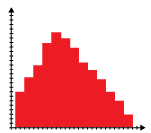
\includegraphics[width=3cm, height=3cm]{histogram_chart}

\subsection{Bar Plot}
Bar plots are usually used to display categorical data along the horizontal axis. That is, discrete data such as products, countries, car types and such. 

Bar within a bar chart are not adjacent. Data on the bar plots are often ordered, in order to enhance chart comprehension. 

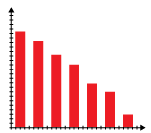
\includegraphics[width=3cm, height=3cm]{bar_chart}

\subsection{Ogive}
An ogive (oh-jive), sometimes called a cumulative frequency chart, is a type of frequency chart that shows cumulative frequencies. In other words, the cumulative percentages are added on the graph from left to right.

An ogive graph plots cumulative frequency on the y-axis and class boundaries along the x-axis. It’s very similar to a histogram, only instead of rectangles, an ogive has a single point marking where the top right of the rectangle would be. 

It is usually easier to create this kind of graph from a frequency table

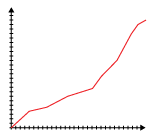
\includegraphics[width=3cm, height=3cm]{ogive_chart}

\subsection{Box and Whisker Plot}
A box and whisker plot is defined as a graphical method of displaying variation in a set of data. It is usually used to display data according to quartile intervals.

BWP are also called: box plot, box and whisker diagram, box and whisker plot with outliers\footnote{"Diagramma a scatola e baffi in italiano"}.

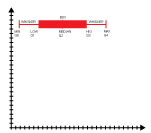
\includegraphics[width=4cm, height=4cm]{box_whisker_chart}

\paragraph{Box and whisker vs candlestick chart}\mbox{} \\
\mbox{} \\
Mathematically speaking there is no difference. Both show an upper and lower boundary and points outside these boundaries. However:
A candlestick chart is mainly used in the finance industry. Its most popular application is to show share price. It is mainly used in the vertical position.

A  box and whisker chart tends to be used in non-finance industries. For example, the level of sales of various stores or inventory levels etc. The box and whisker can be shown horizontally as well as vertically. They are often found with labels showing various statistical informations. 

\subsection{Violin Plot}
A violin plot is a method of plotting numeric data. It is similar to a box plot, with the addition of a rotated kernel density plot on each side.

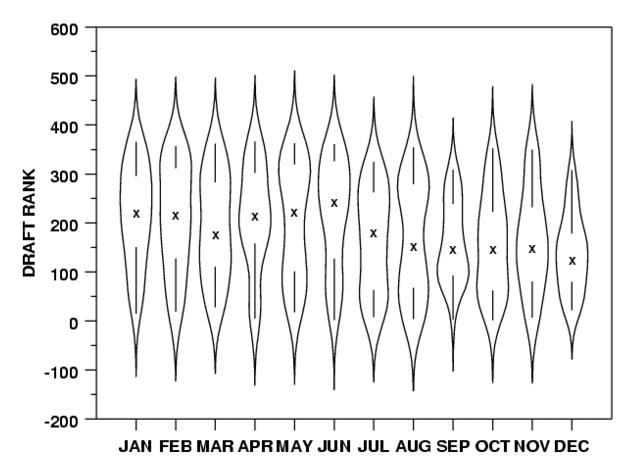
\includegraphics[width=5cm, height=3cm]{violin_chart}

\subsection{KDE Plot}

KDE Plot described as Kernel Density Estimate is used for visualizing the Probability Density of a continuous variable. It depicts the probability density at different values in a continuous variable. We can also plot a single graph for multiple samples which helps in more efficient data visualization.
Kernel density estimates are closely related to histograms, but can be endowed with properties such as smoothness or continuity by using a suitable kernel.

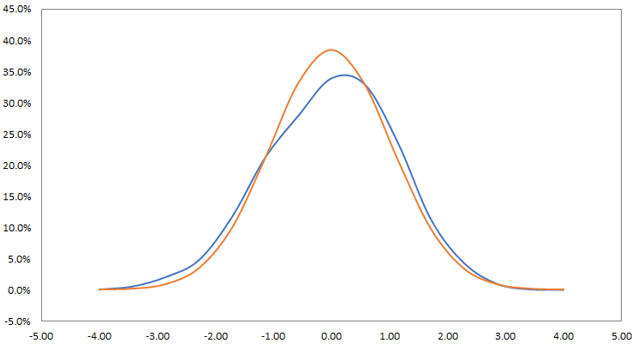
\includegraphics[width=5cm, height=3cm]{kde_chart}
\clearpage

\section{Combinatorics}
Combinatoric is an area of mathematics primarily concerned with counting, both as a means and an end in obtaining results, and certain properties of finite structures. It is closely related to many other areas of mathematics and has many applications ranging from logic to statistical physics and from evolutionary biology to computer science.

\subsection{Factorials}
In mathematics, the factorial of a non-negative integer $n$, denoted by $n!$, is the product of all positive integers less than or equal to $n$. The factorial of $n$ also equals the product of $n$ with the next smaller factorial.

5! = 5 * 4 * 3 * 2 * 1 = 120

An interesting property is also:

$n! = n * (n-1)!$

Example:
5! = 5 * 4! = 120

This leads to:
$\frac{n!}{(n-1)!} = \frac{n(n-1)!}{(n-1)!} = n$

\paragraph{Factorials and 0}\mbox{} \\
\mbox{} \\
Factorials deal only with natural numbers, hence 0 is omitted in the series (otherwise $n! = 0$).

But why 0! = 1 ?

It’s proven that:

$(n-1)! = \frac{n!}{n}$

This means that: \\
4! = 24 \\
3! = 24 / 4 = 6 \\
2! = 6 / 3 = 2 \\
1! = 2 / 2 = 1 \\
0! = 1 / 1 = 1 \\

And, following the same logic: \\
-1! = 1 / 0 = ND \\

that’s why $n!$ if $n \in {N} $ 

\subsection{Permutations}
A permutation of a set of objects is an arrangement of the objects \textbf{in a certain order}. 
Permutations differ from combinations, which are selections of some members of a set regardless of order. 

Usually permutations refer to all the possible arrangements (all the possible permutations of a set of objects). 

Permutations are calculated as factorials $(n!)$

Permutations are relevant when working with numbers, since "575" is not equal to "577" nor "557".

\subsection{Combinations}
A combination is a selection of items from a set that has distinct members, such that the order of selection does not matter (unlike permutations). 
For example, given three fruits, say an apple, an orange and a pear, there are three combinations of two that can be drawn from this set: 
\begin{itemize}
    \item an apple and a pear;
    \item an apple and an orange;
    \item a pear and an orange.
\end{itemize} 
Combinations \textbf{is an unordered selection} of objects from a set of objects.

More formally, a $k-combination$ of a set $S$ is a subset of $k$ distinct elements of $S$.

Combinations are relevant when working with products, or people: apple and orange is equal to orange and apple. A team with Mark and Tom is equal to a team with Tom and Mark.

The number of combinations from a set of $n$ objects taken $k$ a time is:

$\displaystyle C _n ^k = \binom{n}{k} = \frac{n!}{k!(n - k)!}$

\subsubsection{Permutations, Combinations and Dispositions}
\begin{center}
\begin{tabular}{|m{2cm}|c|c|}
\hline
& REPETITION & NO REPETITION (simple) \\ \hline
&&\\[-1em]
Permutations & $\displaystyle n^k$ & \makecell{$\displaystyle \frac{n!}{(n - k)!}$ \\[15pt] where $k = \text{cluster size}$ \\[15pt] $\displaystyle \frac{n!}{k1! * k2! * kn!}$ \\[15pt] where $k = \text{items repeated}$} \\[50pt] \hline
&&\\[-1em]
Combinations & $\displaystyle \frac{(n + k - 1)}{k!(n - 1)!}$ & $\displaystyle \frac{n!}{k!(n - k)!}$ \\[25pt] \hline
&&\\[-1em]
Dispositions & $\displaystyle n^k$ & $\displaystyle \frac{n!}{(n - k)!}$ \\[25pt] 
\hline
\end{tabular}
\end{center}

\paragraph{Examples}\mbox{} \\
\mbox{} \\
\textbf{Permutations with repetitions} \\ 
How many phone numbers of 7 digits can we generate using all the numbers from 0 to 9, allowing every specific case (such as "all zeros" being a valid number)?

$n = \text{[0, 1, 2, 3, 4, 5, 6, 7, 8, 9]} = 10$ \\
$k = \_ \_ \_ \_ \_ \_ \_ = 7$ \\ 
Each slot of k allows 10 combinations, so it’s $n^k = 10^7$

\textbf{Permutations with no repetitions example} \\
Find all the way the word MAMA can be arranged. 

n = 3 \\ 
k1 = 2 (the letter M is repeated 2 times) \\
k2 = 2 (the letter A is repeated 2 times) \\ 
4! / (2! * 2!) = 24 / 4 = 6 \mbox{} \\
\mbox{} \\
How can we arrange 5 students in 3 chairs? \\ 

n = 5 (all the students we have to pick from). \\
k = 3 (seats available). \\
5! / (5 - 3)! = 120 / 2 = 60 \mbox{} \\
\mbox{} \\

\paragraph{When to use permutations, combinations or dispositions? A diagram}\mbox{} \\
\mbox{} \\
Key insight: \\ 
Is the order relevant?
\begin{itemize}
    \item YES = PERMUTATIONS (ex. numbers)
    \item NO = COMBINATIONS (ex. people in teams)
\end{itemize}

\begin{adjustwidth}{-2.0cm}{-3.0cm}

    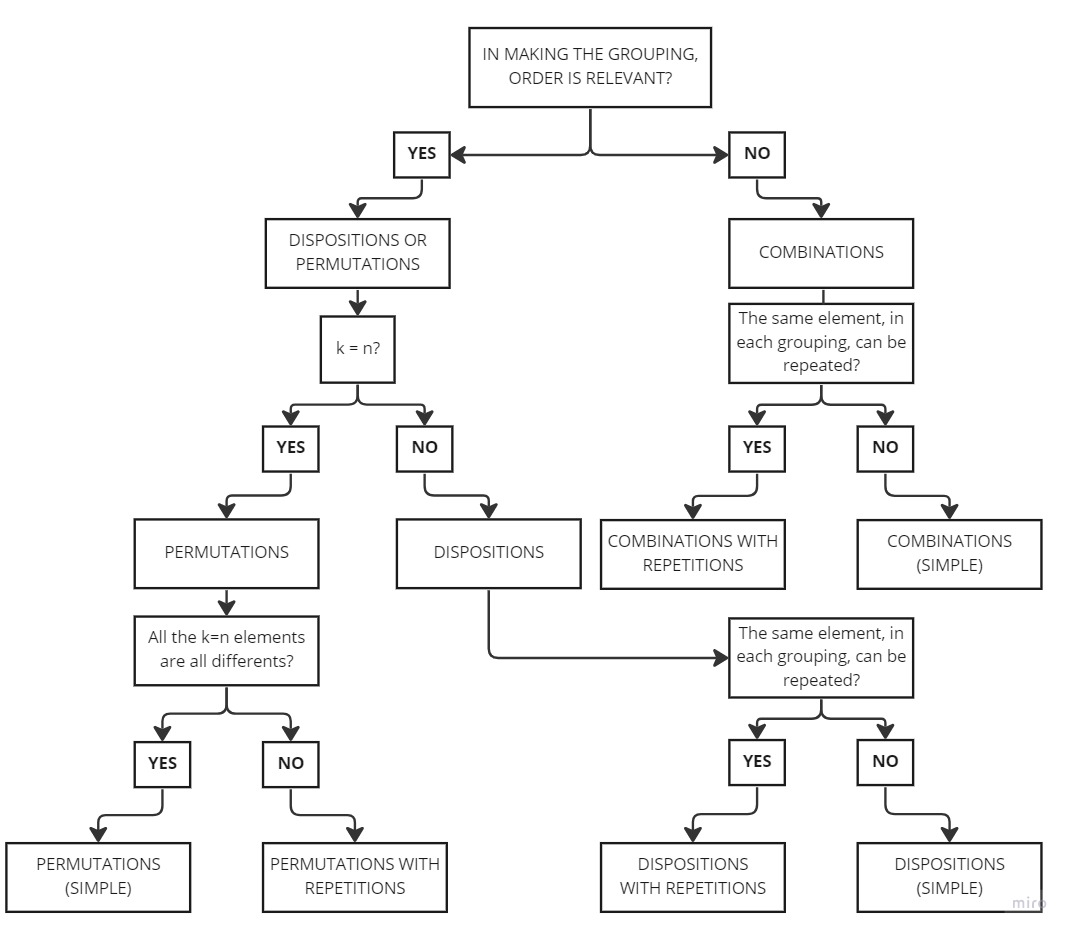
\includegraphics[width=20cm, height=20cm]{stat_diagram}

\end{adjustwidth}
\clearpage

\section{Probability}
Probability is the branch of mathematics that deals with how likely an event is to occur, or how likely is that a given proposition is true.

\paragraph{Probability Notation}\mbox{} \\

\begin{center}
\begin{tabular}{|c|c|c|}
\hline
$P(A)$ & Individual probability & The probability of event $A$ happening \\ \hline
&&\\[-1em]
$P(A')$ & Complement & The probability of event A not happening \\ \hline
&&\\[-1em]
$P(A')$ & Complement & The probability of event A not happening \\ \hline
&&\\[-1em]
$P(A \cup B)$ & Union & \makecell{The probability of both A and B happening for both datasets \\ (all elements of A plus all elements of B).} \\ \hline
&&\\[-1em]
$P(A \cap B)$ & Union & \makecell{The probability of both A and B happening for both datasets \\ (all elements of A plus all elements of B).} \\ \hline
&&\\[-1em]
$P(A | B)$ & Dependent & The probability of A given that B has occurred. \\
\hline
\end{tabular}
\end{center}

\mbox{} \\

\textbf{Example}\\ 
If $P = \{1,3,5,7,9\}$ and $Q = \{2,3,5,7\}$ \\
What are $P \cup Q$, and $P \cap  Q$? \\ 
\mbox{} \\
$P \cup Q = \{1,2,3,5,7,9\}$ \\ 
$P \cap Q = \{3,5,7\}$ \\

\subsection{Simple Probability}
Simple probability define how likely a specific event $A$ is going to happen in the given scenario. 

$P(A) = \text{target events / total events}$ \\
\mbox{} \\
And, consequentially: \\
\mbox{} \\
$P(A') = 1 - P(A)$

\paragraph{Experimental and Expected probability}\mbox{} \\
\mbox{} \\
\begin{itemize}
    \item Experimental probability is the probability resulting from empirical experimentations, such as flipping a coin 100 times and recording the results in a datasheet.
    \item Expected probability is the theoretical probability coming from applying the probability formula to the scenario.
\end{itemize}

The expected probability of having head over a coin toss is 50\%. However over a 100 tosses, the experimental probability may vary (ex. resulting in 30\% heads).

\paragraph{Law of Large Numbers}\mbox{} \\
\mbox{} \\
The law of large numbers, or Bernoulli's theorem (since its first formulation is due to Jakob Bernoulli), describes the behavior of the mean of a sequence of $n$ trials of a random variable, independent and characterized by the same probability distribution (n measurements of the same magnitude, $n$ tosses of the same coin, etc.), as the numerosity of the sequence itself $n$ tends to infinity.

\subsubsection{Probability Addition Rule}
If A and B are two events in a probability experiment, then the probability that either one of the events will occur is: \\ 
\mbox{} \\
$P(A or B)=P(A)+P(B)−P(A and B)$ \\ 
\mbox{} \\
Or, with sets notation as: \\ 
\mbox{} \\
$P(A \cup B) = P(A)+P(B)−P(A \cap B)$ 

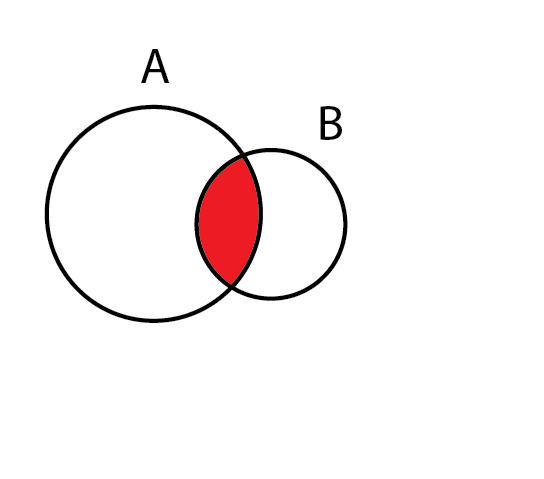
\includegraphics[width=3.5cm, height=3cm]{intersection}

If A and B are two mutually exclusive events, \\ 
$P(A \cap B) = 0$. Then the probability that either one of the events will occur is: \\
\mbox{} \\
$P(A or B)=P(A)+P(B)$ \\
\mbox{} \\
Or, with sets notation as: \\ 
\mbox{} \\
$P(A \cup B)=P(A) + P(B)$ \\ 

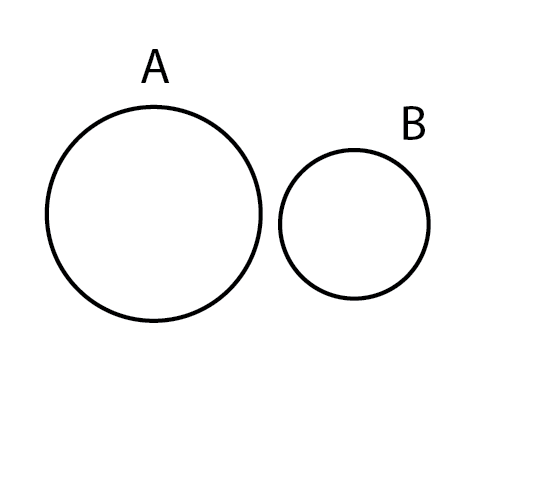
\includegraphics[width=3.5cm, height=3cm]{independent}

\textbf{Fundamental rule for addition or product in probability calculation} \\

\begin{itemize}
    \item Given two \textbf{independent} events, the probability of them \textbf{occurring both} is given by the \textbf{product} of the individual probabilities. 
    \begin{itemize}
        \item Example: having a head out of two coin flips.
    \end{itemize}
    \item The probability of two or more \textbf{alternative} events occurring is equal to the \textbf{sum} of the individual probabilities. 
    \begin{itemize}
        \item Example: having 1 or 2 out of a dice roll.
    \end{itemize}
\end{itemize}

\subsubsection{Conditional Probability for Independent and Dependent Events}
\textbf{Independent event probability} \\ 
The probability of A and B happening. \\
\mbox{} \\
$P(A \cap B) = P(A) * P(B)$ \\ 
\mbox{} \\
Tossing two coins A and B, what is the probability of having two head values? \\ 
Coins are independent each other, so: \\ 
\mbox{} \\
$P(A \cap B) = 1 / 2 * 1 / 2 = 1 / 4 $ \\ 
\mbox{} \\
Defective rate in a production line is 2\%. \\ 
What is the probability of having 3 defective products in a row?\\
\mbox{} \\
$P(A \cap B \cap  C) = 2 / 100 * 2 / 100 * 2 / 100 = \frac{8}{100^3} = 1 / 125'000$ \\ 
\mbox{} \\
\textbf{Dependent event probability}
\mbox{} \\
The probability of A and B, given that A has already occurred. \\ 
\mbox{} \\
$P(A \cap B) = P(A) * P(B | A)$ \\ 
\mbox{} \\
What’s the probability of drafting two Kings in a row from a standard deck of cards? \\

$P(A \cap B) = 4 / 52 * 3 / 51  = 1 / 13 * 1 / 17 = 1 / 221$

\textbf{Reminder}

If $P(B) = P(B | A)$ then the events must be independent.

\subsection{Bayes Theorem}
Bayes' theorem describes the probability of an event, based on prior knowledge of conditions that might be related to the event. 

$\displaystyle P(A\mid B)={\frac {P(B\mid A)P(A)}{P(B)}}$ \\ 

Where: 
\begin{itemize}
    \item $A$ and $B$ are events and $P(B) \neq 0 $.
    \item $P(A)$ is the probability of event $A$.
    \item $P(B)$ is the probability of event $B$.
    \item $P(A | B)$ is the probability of observing event $A$ if $B$ is true.
    \item $P(B | A)$ is the probability of observing event $B$ if $A$ is true.
\end{itemize}

\paragraph{Example 1.}\mbox{} \\
\mbox{} \\
We have two assembly lines, 1 and 2. \\ 
Line 1 has a defective rate of 3\%, Line 2 of 1\%. \\ 
Given a defective part, what is the probability that it came from line 1? \\ 
\mbox{} \\
Let’s call:
\begin{itemize}
    \item $P(B)$ the probability of a product being defective.
    \item $P(A)$ the probability of a product coming from line 1.
\end{itemize}
Hence: \\ 
\mbox{} \\
$P(A) = 1 / 2$ \\  
(with the available data, we must assume we have a 50\% likelihood from two lines). 

$P(B | A)$ = probability of $B$(defect) if $A$(product is coming from line 1) has occurred = $3 / 100$ (this is the info provided by the context already).

$P(B)$ = overall probability of having a defective product = $[(1 / 2) * (3 / 100)] + [(1 / 2) * (1 / 100)] =   3 / 200 + 1/ 200 = 4 / 200 = 1 / 50$

Applying Bayes Theorem, then:

$P(A | B) = [(3 / 100) * (1 / 2)] / (1 / 50) = (3 / 200) / (1 / 50) = (3 / 200) * (50 / 1) = 150 / 200 = 3 / 4 = 75\% $

\paragraph{Example 2.}\mbox{} \\
\mbox{} \\
You’re tested for a disease that occurs 1 out of 1’000 people. \\ 
Test accuracy is 99\%. \\ 
You are tested positive. \\ 
What is the change you actually have the disease? \\ 
\mbox{} \\
\begin{itemize}
    \item Population: $1'000$
    \item Incidence: $(1/1’000) = 0.001$
    \item Accuracy: 99\%
    \item False positive \ negative: $(100\% - 99\%) = 1\%$
\end{itemize}

\begin{center}
\begin{tabular}{|c|c|c|c|}
\hline
 & SICK & NOT SICK & TOTAL \\ \hline
&&&\\[-1em]
TESTED POS & 0.99[1] & 9.99[3] & 10.98 \\ \hline
&&&\\[-1em]
TESTED NEG & 0.01[2] & 989.01[4] & 989.02 \\ \hline
&&&\\[-1em]
TOTAL & 1 & 999 & 1'000 \\ 
\hline
\end{tabular}
\end{center}
\mbox{} \\  
{[1]} = $1’000 * 0.001 * 99\%$ \\ 
{[2]} = $1’000 * 0.001 * 1\%$ \\ 
{[3]} = $(1’000 * (1 - 0.001)) * 1\%$ \\ 
{[4]} = $(1’000 * (1 - 0.001)) * 99\%$ \\
\mbox{} \\
$P(A)$ = probability of being sick = $0.001$ \\ 
$P(B)$ = probability of having a positive test = $10.98 / 1’000$ \\ 
$P(B|A)$ = probability of having a positive test being sick = $0.99$ \\ 
$P(A|B)$ = probability of being sick having a positive test = $10.98 / 0.99$ (or applying Bayesian formula) = $9\%$ \\ 



\end{document}




